\documentclass[twoside]{book}

% Packages required by doxygen
\usepackage{fixltx2e}
\usepackage{calc}
\usepackage{doxygen}
\usepackage[export]{adjustbox} % also loads graphicx
\usepackage{graphicx}
\usepackage[utf8]{inputenc}
\usepackage{makeidx}
\usepackage{multicol}
\usepackage{multirow}
\PassOptionsToPackage{warn}{textcomp}
\usepackage{textcomp}
\usepackage[nointegrals]{wasysym}
\usepackage[table]{xcolor}

% Font selection
\usepackage[T1]{fontenc}
\usepackage[scaled=.90]{helvet}
\usepackage{courier}
\usepackage{amssymb}
\usepackage{sectsty}
\renewcommand{\familydefault}{\sfdefault}
\allsectionsfont{%
  \fontseries{bc}\selectfont%
  \color{darkgray}%
}
\renewcommand{\DoxyLabelFont}{%
  \fontseries{bc}\selectfont%
  \color{darkgray}%
}
\newcommand{\+}{\discretionary{\mbox{\scriptsize$\hookleftarrow$}}{}{}}

% Page & text layout
\usepackage{geometry}
\geometry{%
  a4paper,%
  top=2.5cm,%
  bottom=2.5cm,%
  left=2.5cm,%
  right=2.5cm%
}
\tolerance=750
\hfuzz=15pt
\hbadness=750
\setlength{\emergencystretch}{15pt}
\setlength{\parindent}{0cm}
\setlength{\parskip}{3ex plus 2ex minus 2ex}
\makeatletter
\renewcommand{\paragraph}{%
  \@startsection{paragraph}{4}{0ex}{-1.0ex}{1.0ex}{%
    \normalfont\normalsize\bfseries\SS@parafont%
  }%
}
\renewcommand{\subparagraph}{%
  \@startsection{subparagraph}{5}{0ex}{-1.0ex}{1.0ex}{%
    \normalfont\normalsize\bfseries\SS@subparafont%
  }%
}
\makeatother

% Headers & footers
\usepackage{fancyhdr}
\pagestyle{fancyplain}
\fancyhead[LE]{\fancyplain{}{\bfseries\thepage}}
\fancyhead[CE]{\fancyplain{}{}}
\fancyhead[RE]{\fancyplain{}{\bfseries\leftmark}}
\fancyhead[LO]{\fancyplain{}{\bfseries\rightmark}}
\fancyhead[CO]{\fancyplain{}{}}
\fancyhead[RO]{\fancyplain{}{\bfseries\thepage}}
\fancyfoot[LE]{\fancyplain{}{}}
\fancyfoot[CE]{\fancyplain{}{}}
\fancyfoot[RE]{\fancyplain{}{\bfseries\scriptsize Generated by Doxygen }}
\fancyfoot[LO]{\fancyplain{}{\bfseries\scriptsize Generated by Doxygen }}
\fancyfoot[CO]{\fancyplain{}{}}
\fancyfoot[RO]{\fancyplain{}{}}
\renewcommand{\footrulewidth}{0.4pt}
\renewcommand{\chaptermark}[1]{%
  \markboth{#1}{}%
}
\renewcommand{\sectionmark}[1]{%
  \markright{\thesection\ #1}%
}

% Indices & bibliography
\usepackage{natbib}
\usepackage[titles]{tocloft}
\setcounter{tocdepth}{3}
\setcounter{secnumdepth}{5}
\makeindex

% Hyperlinks (required, but should be loaded last)
\usepackage{ifpdf}
\ifpdf
  \usepackage[pdftex,pagebackref=true]{hyperref}
\else
  \usepackage[ps2pdf,pagebackref=true]{hyperref}
\fi
\hypersetup{%
  colorlinks=true,%
  linkcolor=blue,%
  citecolor=blue,%
  unicode%
}

% Custom commands
\newcommand{\clearemptydoublepage}{%
  \newpage{\pagestyle{empty}\cleardoublepage}%
}

\usepackage{caption}
\captionsetup{labelsep=space,justification=centering,font={bf},singlelinecheck=off,skip=4pt,position=top}

%===== C O N T E N T S =====

\begin{document}

% Titlepage & ToC
\hypersetup{pageanchor=false,
             bookmarksnumbered=true,
             pdfencoding=unicode
            }
\pagenumbering{roman}
\begin{titlepage}
\vspace*{7cm}
\begin{center}%
{\Large My Project }\\
\vspace*{1cm}
{\large Generated by Doxygen 1.8.11}\\
\end{center}
\end{titlepage}
\clearemptydoublepage
\tableofcontents
\clearemptydoublepage
\pagenumbering{arabic}
\hypersetup{pageanchor=true}

%--- Begin generated contents ---
\chapter{Namespace Index}
\section{Namespace List}
Here is a list of all namespaces with brief descriptions\+:\begin{DoxyCompactList}
\item\contentsline{section}{\hyperlink{namespacequeuesavitch}{queuesavitch} }{\pageref{namespacequeuesavitch}}{}
\end{DoxyCompactList}

\chapter{Hierarchical Index}
\section{Class Hierarchy}
This inheritance list is sorted roughly, but not completely, alphabetically\+:\begin{DoxyCompactList}
\item \contentsline{section}{Fruit}{\pageref{classFruit}}{}
\begin{DoxyCompactList}
\item \contentsline{section}{Apple}{\pageref{classApple}}{}
\item \contentsline{section}{Grape}{\pageref{classGrape}}{}
\item \contentsline{section}{Orange}{\pageref{classOrange}}{}
\end{DoxyCompactList}
\item \contentsline{section}{List}{\pageref{classList}}{}
\item \contentsline{section}{List\+:\+:Node}{\pageref{structList_1_1Node}}{}
\end{DoxyCompactList}

\chapter{Class Index}
\section{Class List}
Here are the classes, structs, unions and interfaces with brief descriptions\+:\begin{DoxyCompactList}
\item\contentsline{section}{\hyperlink{structnode}{node} }{\pageref{structnode}}{}
\item\contentsline{section}{\hyperlink{structnode1}{node1} }{\pageref{structnode1}}{}
\item\contentsline{section}{\hyperlink{structnode__info}{node\+\_\+info} }{\pageref{structnode__info}}{}
\end{DoxyCompactList}

\chapter{File Index}
\section{File List}
Here is a list of all files with brief descriptions\+:\begin{DoxyCompactList}
\item\contentsline{section}{\hyperlink{Lab1_8c}{Lab1.\+c} }{\pageref{Lab1_8c}}{}
\end{DoxyCompactList}

\chapter{Namespace Documentation}
\hypertarget{namespacewikibooks__design__patterns}{}\section{wikibooks\+\_\+design\+\_\+patterns Namespace Reference}
\label{namespacewikibooks__design__patterns}\index{wikibooks\+\_\+design\+\_\+patterns@{wikibooks\+\_\+design\+\_\+patterns}}
\subsection*{Classes}
\begin{DoxyCompactItemize}
\item 
class \hyperlink{classwikibooks__design__patterns_1_1Evaluator}{Evaluator}
\item 
struct \hyperlink{structwikibooks__design__patterns_1_1Expression}{Expression}
\item 
class \hyperlink{classwikibooks__design__patterns_1_1Minus}{Minus}
\item 
class \hyperlink{classwikibooks__design__patterns_1_1Number}{Number}
\item 
class \hyperlink{classwikibooks__design__patterns_1_1Plus}{Plus}
\item 
class \hyperlink{classwikibooks__design__patterns_1_1Variable}{Variable}
\end{DoxyCompactItemize}
\subsection*{Typedefs}
\begin{DoxyCompactItemize}
\item 
typedef std\+::string \hyperlink{namespacewikibooks__design__patterns_a603d2591ea56686888d0e4389481a453}{String}
\item 
typedef std\+::map$<$ \hyperlink{namespacewikibooks__design__patterns_a603d2591ea56686888d0e4389481a453}{String}, \hyperlink{structwikibooks__design__patterns_1_1Expression}{Expression} $\ast$ $>$ \hyperlink{namespacewikibooks__design__patterns_adf1889a865861dea765d8a115cc66ae9}{Map}
\item 
typedef std\+::list$<$ \hyperlink{structwikibooks__design__patterns_1_1Expression}{Expression} $\ast$ $>$ \hyperlink{namespacewikibooks__design__patterns_a3247979de240b19de03793d4ec6ede0e}{Stack}
\end{DoxyCompactItemize}


\subsection{Typedef Documentation}
\index{wikibooks\+\_\+design\+\_\+patterns@{wikibooks\+\_\+design\+\_\+patterns}!Map@{Map}}
\index{Map@{Map}!wikibooks\+\_\+design\+\_\+patterns@{wikibooks\+\_\+design\+\_\+patterns}}
\subsubsection[{\texorpdfstring{Map}{Map}}]{\setlength{\rightskip}{0pt plus 5cm}typedef std\+::map$<${\bf String},{\bf Expression}$\ast$$>$ {\bf wikibooks\+\_\+design\+\_\+patterns\+::\+Map}}\hypertarget{namespacewikibooks__design__patterns_adf1889a865861dea765d8a115cc66ae9}{}\label{namespacewikibooks__design__patterns_adf1889a865861dea765d8a115cc66ae9}
\index{wikibooks\+\_\+design\+\_\+patterns@{wikibooks\+\_\+design\+\_\+patterns}!Stack@{Stack}}
\index{Stack@{Stack}!wikibooks\+\_\+design\+\_\+patterns@{wikibooks\+\_\+design\+\_\+patterns}}
\subsubsection[{\texorpdfstring{Stack}{Stack}}]{\setlength{\rightskip}{0pt plus 5cm}typedef std\+::list$<${\bf Expression}$\ast$$>$ {\bf wikibooks\+\_\+design\+\_\+patterns\+::\+Stack}}\hypertarget{namespacewikibooks__design__patterns_a3247979de240b19de03793d4ec6ede0e}{}\label{namespacewikibooks__design__patterns_a3247979de240b19de03793d4ec6ede0e}
\index{wikibooks\+\_\+design\+\_\+patterns@{wikibooks\+\_\+design\+\_\+patterns}!String@{String}}
\index{String@{String}!wikibooks\+\_\+design\+\_\+patterns@{wikibooks\+\_\+design\+\_\+patterns}}
\subsubsection[{\texorpdfstring{String}{String}}]{\setlength{\rightskip}{0pt plus 5cm}typedef std\+::string {\bf wikibooks\+\_\+design\+\_\+patterns\+::\+String}}\hypertarget{namespacewikibooks__design__patterns_a603d2591ea56686888d0e4389481a453}{}\label{namespacewikibooks__design__patterns_a603d2591ea56686888d0e4389481a453}

\chapter{Class Documentation}
\hypertarget{classwikibooks__design__patterns_1_1Evaluator}{}\section{wikibooks\+\_\+design\+\_\+patterns\+:\+:Evaluator Class Reference}
\label{classwikibooks__design__patterns_1_1Evaluator}\index{wikibooks\+\_\+design\+\_\+patterns\+::\+Evaluator@{wikibooks\+\_\+design\+\_\+patterns\+::\+Evaluator}}


Inheritance diagram for wikibooks\+\_\+design\+\_\+patterns\+:\+:Evaluator\+:
\nopagebreak
\begin{figure}[H]
\begin{center}
\leavevmode
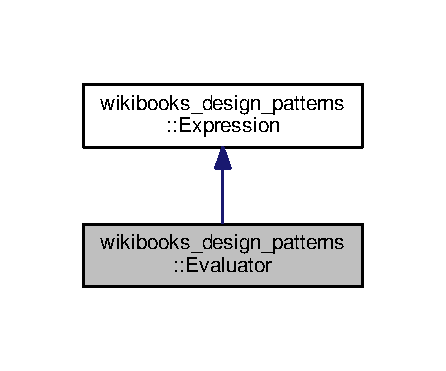
\includegraphics[width=214pt]{classwikibooks__design__patterns_1_1Evaluator__inherit__graph}
\end{center}
\end{figure}


Collaboration diagram for wikibooks\+\_\+design\+\_\+patterns\+:\+:Evaluator\+:
\nopagebreak
\begin{figure}[H]
\begin{center}
\leavevmode
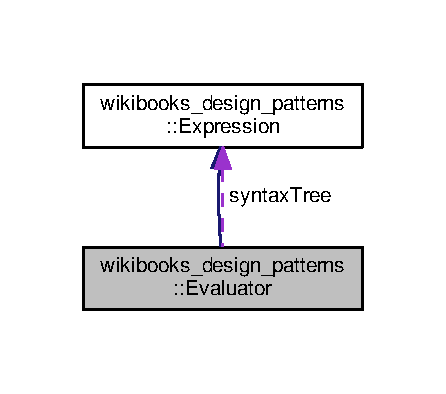
\includegraphics[width=214pt]{classwikibooks__design__patterns_1_1Evaluator__coll__graph}
\end{center}
\end{figure}
\subsection*{Public Member Functions}
\begin{DoxyCompactItemize}
\item 
\hyperlink{classwikibooks__design__patterns_1_1Evaluator_aa9d884c25c638c6bf4b9cc6048b6c0e6}{Evaluator} (\hyperlink{namespacewikibooks__design__patterns_a603d2591ea56686888d0e4389481a453}{String} expression)
\item 
\hyperlink{classwikibooks__design__patterns_1_1Evaluator_a8d8907ba7b681cdd76e53d451c2d1a19}{$\sim$\+Evaluator} ()
\item 
int \hyperlink{classwikibooks__design__patterns_1_1Evaluator_aa7ba308eda08d2fbff093f684f7a0832}{interpret} (\hyperlink{namespacewikibooks__design__patterns_adf1889a865861dea765d8a115cc66ae9}{Map} context)
\end{DoxyCompactItemize}
\subsection*{Private Attributes}
\begin{DoxyCompactItemize}
\item 
\hyperlink{structwikibooks__design__patterns_1_1Expression}{Expression} $\ast$ \hyperlink{classwikibooks__design__patterns_1_1Evaluator_a22439cc7dc84a90b755c2955c8c4ac74}{syntax\+Tree}
\end{DoxyCompactItemize}


\subsection{Constructor \& Destructor Documentation}
\index{wikibooks\+\_\+design\+\_\+patterns\+::\+Evaluator@{wikibooks\+\_\+design\+\_\+patterns\+::\+Evaluator}!Evaluator@{Evaluator}}
\index{Evaluator@{Evaluator}!wikibooks\+\_\+design\+\_\+patterns\+::\+Evaluator@{wikibooks\+\_\+design\+\_\+patterns\+::\+Evaluator}}
\subsubsection[{\texorpdfstring{Evaluator(\+String expression)}{Evaluator(String expression)}}]{\setlength{\rightskip}{0pt plus 5cm}wikibooks\+\_\+design\+\_\+patterns\+::\+Evaluator\+::\+Evaluator (
\begin{DoxyParamCaption}
\item[{{\bf String}}]{expression}
\end{DoxyParamCaption}
)\hspace{0.3cm}{\ttfamily [inline]}}\hypertarget{classwikibooks__design__patterns_1_1Evaluator_aa9d884c25c638c6bf4b9cc6048b6c0e6}{}\label{classwikibooks__design__patterns_1_1Evaluator_aa9d884c25c638c6bf4b9cc6048b6c0e6}

\begin{DoxyCode}
83                                 \{
84         \hyperlink{namespacewikibooks__design__patterns_a3247979de240b19de03793d4ec6ede0e}{Stack} expressionStack;
85 
86     \textcolor{keywordtype}{size\_t} last = 0;
87     \textcolor{keywordflow}{for} (\textcolor{keywordtype}{size\_t} next = 0; String::npos != last; last = (String::npos == next) ? next : (1+next)) \{
88         next = expression.find(\textcolor{charliteral}{' '}, last);
89         \hyperlink{namespacewikibooks__design__patterns_a603d2591ea56686888d0e4389481a453}{String} token( expression.substr(last, (String::npos == next) ? (expression.length()-last) : (
      next-last)));
90 
91             \textcolor{keywordflow}{if}  (token == \textcolor{stringliteral}{"+"}) \{
92         \hyperlink{structwikibooks__design__patterns_1_1Expression}{Expression}* right = expressionStack.back(); expressionStack.pop\_back();
93                 \hyperlink{structwikibooks__design__patterns_1_1Expression}{Expression}* left = expressionStack.back(); expressionStack.pop\_back();
94                 \hyperlink{structwikibooks__design__patterns_1_1Expression}{Expression}* subExpression = \textcolor{keyword}{new} \hyperlink{classwikibooks__design__patterns_1_1Plus}{Plus}(right, left);
95                 expressionStack.push\_back( subExpression );
96             \}
97             \textcolor{keywordflow}{else} \textcolor{keywordflow}{if} (token == \textcolor{stringliteral}{"-"}) \{
98                 \textcolor{comment}{// it's necessary remove first the right operand from the stack}
99                 \hyperlink{structwikibooks__design__patterns_1_1Expression}{Expression}* right = expressionStack.back(); expressionStack.pop\_back();
100                 \textcolor{comment}{// ..and after the left one}
101                 \hyperlink{structwikibooks__design__patterns_1_1Expression}{Expression}* left = expressionStack.back(); expressionStack.pop\_back();
102                 \hyperlink{structwikibooks__design__patterns_1_1Expression}{Expression}* subExpression = \textcolor{keyword}{new} \hyperlink{classwikibooks__design__patterns_1_1Minus}{Minus}(left, right);
103                 expressionStack.push\_back( subExpression );
104             \}
105             \textcolor{keywordflow}{else}                        
106                 expressionStack.push\_back( \textcolor{keyword}{new} \hyperlink{classwikibooks__design__patterns_1_1Variable}{Variable}(token) );
107         \}
108 
109         \hyperlink{classwikibooks__design__patterns_1_1Evaluator_a22439cc7dc84a90b755c2955c8c4ac74}{syntaxTree} = expressionStack.back(); expressionStack.pop\_back();
110     \}
\end{DoxyCode}
\index{wikibooks\+\_\+design\+\_\+patterns\+::\+Evaluator@{wikibooks\+\_\+design\+\_\+patterns\+::\+Evaluator}!````~Evaluator@{$\sim$\+Evaluator}}
\index{````~Evaluator@{$\sim$\+Evaluator}!wikibooks\+\_\+design\+\_\+patterns\+::\+Evaluator@{wikibooks\+\_\+design\+\_\+patterns\+::\+Evaluator}}
\subsubsection[{\texorpdfstring{$\sim$\+Evaluator()}{~Evaluator()}}]{\setlength{\rightskip}{0pt plus 5cm}wikibooks\+\_\+design\+\_\+patterns\+::\+Evaluator\+::$\sim$\+Evaluator (
\begin{DoxyParamCaption}
{}
\end{DoxyParamCaption}
)\hspace{0.3cm}{\ttfamily [inline]}}\hypertarget{classwikibooks__design__patterns_1_1Evaluator_a8d8907ba7b681cdd76e53d451c2d1a19}{}\label{classwikibooks__design__patterns_1_1Evaluator_a8d8907ba7b681cdd76e53d451c2d1a19}

\begin{DoxyCode}
112                   \{
113     \textcolor{keyword}{delete} \hyperlink{classwikibooks__design__patterns_1_1Evaluator_a22439cc7dc84a90b755c2955c8c4ac74}{syntaxTree};
114      \}
\end{DoxyCode}


\subsection{Member Function Documentation}
\index{wikibooks\+\_\+design\+\_\+patterns\+::\+Evaluator@{wikibooks\+\_\+design\+\_\+patterns\+::\+Evaluator}!interpret@{interpret}}
\index{interpret@{interpret}!wikibooks\+\_\+design\+\_\+patterns\+::\+Evaluator@{wikibooks\+\_\+design\+\_\+patterns\+::\+Evaluator}}
\subsubsection[{\texorpdfstring{interpret(\+Map context)}{interpret(Map context)}}]{\setlength{\rightskip}{0pt plus 5cm}int wikibooks\+\_\+design\+\_\+patterns\+::\+Evaluator\+::interpret (
\begin{DoxyParamCaption}
\item[{{\bf Map}}]{context}
\end{DoxyParamCaption}
)\hspace{0.3cm}{\ttfamily [inline]}, {\ttfamily [virtual]}}\hypertarget{classwikibooks__design__patterns_1_1Evaluator_aa7ba308eda08d2fbff093f684f7a0832}{}\label{classwikibooks__design__patterns_1_1Evaluator_aa7ba308eda08d2fbff093f684f7a0832}


Implements \hyperlink{structwikibooks__design__patterns_1_1Expression_a3723a35bb367b43edf806be72385c680}{wikibooks\+\_\+design\+\_\+patterns\+::\+Expression}.


\begin{DoxyCode}
116                                \{
117         \textcolor{keywordflow}{return} \hyperlink{classwikibooks__design__patterns_1_1Evaluator_a22439cc7dc84a90b755c2955c8c4ac74}{syntaxTree}->\hyperlink{structwikibooks__design__patterns_1_1Expression_a3723a35bb367b43edf806be72385c680}{interpret}(context);
118     \}
\end{DoxyCode}


Here is the call graph for this function\+:
\nopagebreak
\begin{figure}[H]
\begin{center}
\leavevmode
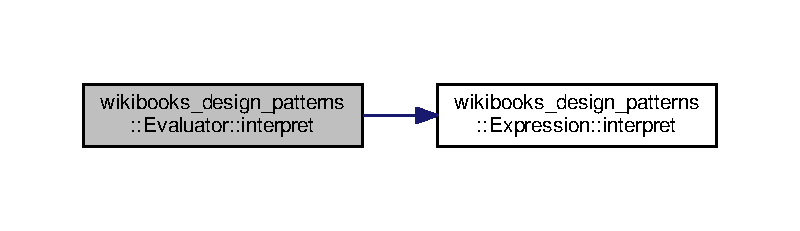
\includegraphics[width=350pt]{classwikibooks__design__patterns_1_1Evaluator_aa7ba308eda08d2fbff093f684f7a0832_cgraph}
\end{center}
\end{figure}




\subsection{Member Data Documentation}
\index{wikibooks\+\_\+design\+\_\+patterns\+::\+Evaluator@{wikibooks\+\_\+design\+\_\+patterns\+::\+Evaluator}!syntax\+Tree@{syntax\+Tree}}
\index{syntax\+Tree@{syntax\+Tree}!wikibooks\+\_\+design\+\_\+patterns\+::\+Evaluator@{wikibooks\+\_\+design\+\_\+patterns\+::\+Evaluator}}
\subsubsection[{\texorpdfstring{syntax\+Tree}{syntaxTree}}]{\setlength{\rightskip}{0pt plus 5cm}{\bf Expression}$\ast$ wikibooks\+\_\+design\+\_\+patterns\+::\+Evaluator\+::syntax\+Tree\hspace{0.3cm}{\ttfamily [private]}}\hypertarget{classwikibooks__design__patterns_1_1Evaluator_a22439cc7dc84a90b755c2955c8c4ac74}{}\label{classwikibooks__design__patterns_1_1Evaluator_a22439cc7dc84a90b755c2955c8c4ac74}


The documentation for this class was generated from the following file\+:\begin{DoxyCompactItemize}
\item 
\hyperlink{Interpreter_8cpp}{Interpreter.\+cpp}\end{DoxyCompactItemize}

\hypertarget{structwikibooks__design__patterns_1_1Expression}{}\section{wikibooks\+\_\+design\+\_\+patterns\+:\+:Expression Struct Reference}
\label{structwikibooks__design__patterns_1_1Expression}\index{wikibooks\+\_\+design\+\_\+patterns\+::\+Expression@{wikibooks\+\_\+design\+\_\+patterns\+::\+Expression}}


Inheritance diagram for wikibooks\+\_\+design\+\_\+patterns\+:\+:Expression\+:
\nopagebreak
\begin{figure}[H]
\begin{center}
\leavevmode
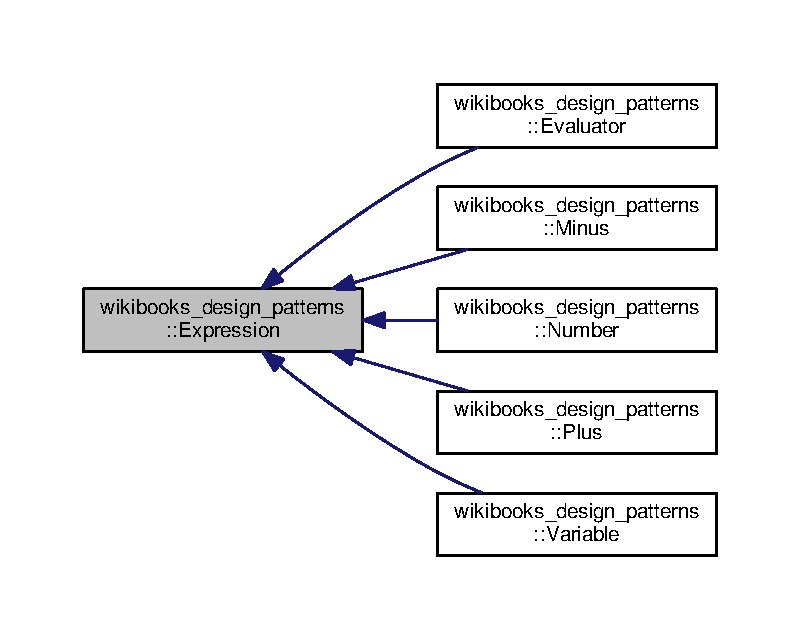
\includegraphics[width=350pt]{structwikibooks__design__patterns_1_1Expression__inherit__graph}
\end{center}
\end{figure}
\subsection*{Public Member Functions}
\begin{DoxyCompactItemize}
\item 
virtual int \hyperlink{structwikibooks__design__patterns_1_1Expression_a3723a35bb367b43edf806be72385c680}{interpret} (\hyperlink{namespacewikibooks__design__patterns_adf1889a865861dea765d8a115cc66ae9}{Map} variables)=0
\item 
virtual \hyperlink{structwikibooks__design__patterns_1_1Expression_a21baa3deef8317373259172c3fcd78ec}{$\sim$\+Expression} ()
\end{DoxyCompactItemize}


\subsection{Constructor \& Destructor Documentation}
\index{wikibooks\+\_\+design\+\_\+patterns\+::\+Expression@{wikibooks\+\_\+design\+\_\+patterns\+::\+Expression}!````~Expression@{$\sim$\+Expression}}
\index{````~Expression@{$\sim$\+Expression}!wikibooks\+\_\+design\+\_\+patterns\+::\+Expression@{wikibooks\+\_\+design\+\_\+patterns\+::\+Expression}}
\subsubsection[{\texorpdfstring{$\sim$\+Expression()}{~Expression()}}]{\setlength{\rightskip}{0pt plus 5cm}virtual wikibooks\+\_\+design\+\_\+patterns\+::\+Expression\+::$\sim$\+Expression (
\begin{DoxyParamCaption}
{}
\end{DoxyParamCaption}
)\hspace{0.3cm}{\ttfamily [inline]}, {\ttfamily [virtual]}}\hypertarget{structwikibooks__design__patterns_1_1Expression_a21baa3deef8317373259172c3fcd78ec}{}\label{structwikibooks__design__patterns_1_1Expression_a21baa3deef8317373259172c3fcd78ec}

\begin{DoxyCode}
18 \{\}
\end{DoxyCode}


\subsection{Member Function Documentation}
\index{wikibooks\+\_\+design\+\_\+patterns\+::\+Expression@{wikibooks\+\_\+design\+\_\+patterns\+::\+Expression}!interpret@{interpret}}
\index{interpret@{interpret}!wikibooks\+\_\+design\+\_\+patterns\+::\+Expression@{wikibooks\+\_\+design\+\_\+patterns\+::\+Expression}}
\subsubsection[{\texorpdfstring{interpret(\+Map variables)=0}{interpret(Map variables)=0}}]{\setlength{\rightskip}{0pt plus 5cm}virtual int wikibooks\+\_\+design\+\_\+patterns\+::\+Expression\+::interpret (
\begin{DoxyParamCaption}
\item[{{\bf Map}}]{variables}
\end{DoxyParamCaption}
)\hspace{0.3cm}{\ttfamily [pure virtual]}}\hypertarget{structwikibooks__design__patterns_1_1Expression_a3723a35bb367b43edf806be72385c680}{}\label{structwikibooks__design__patterns_1_1Expression_a3723a35bb367b43edf806be72385c680}


Implemented in \hyperlink{classwikibooks__design__patterns_1_1Evaluator_aa7ba308eda08d2fbff093f684f7a0832}{wikibooks\+\_\+design\+\_\+patterns\+::\+Evaluator}, \hyperlink{classwikibooks__design__patterns_1_1Variable_a4b0fe47e343d6991a62ee6b0d2179e2f}{wikibooks\+\_\+design\+\_\+patterns\+::\+Variable}, \hyperlink{classwikibooks__design__patterns_1_1Minus_a6f2e1d5e4281ecee45dff5859af3978f}{wikibooks\+\_\+design\+\_\+patterns\+::\+Minus}, \hyperlink{classwikibooks__design__patterns_1_1Plus_a014d62447a10ada652b67da3fd2d6e4a}{wikibooks\+\_\+design\+\_\+patterns\+::\+Plus}, and \hyperlink{classwikibooks__design__patterns_1_1Number_aed3e0a829546568864db2b8e5b667c72}{wikibooks\+\_\+design\+\_\+patterns\+::\+Number}.



The documentation for this struct was generated from the following file\+:\begin{DoxyCompactItemize}
\item 
\hyperlink{Interpreter_8cpp}{Interpreter.\+cpp}\end{DoxyCompactItemize}

\hypertarget{classwikibooks__design__patterns_1_1Minus}{}\section{wikibooks\+\_\+design\+\_\+patterns\+:\+:Minus Class Reference}
\label{classwikibooks__design__patterns_1_1Minus}\index{wikibooks\+\_\+design\+\_\+patterns\+::\+Minus@{wikibooks\+\_\+design\+\_\+patterns\+::\+Minus}}


Inheritance diagram for wikibooks\+\_\+design\+\_\+patterns\+:\+:Minus\+:
\nopagebreak
\begin{figure}[H]
\begin{center}
\leavevmode
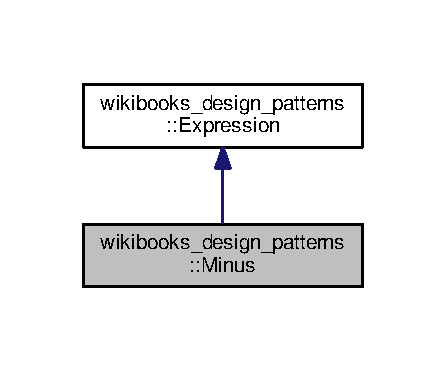
\includegraphics[width=214pt]{classwikibooks__design__patterns_1_1Minus__inherit__graph}
\end{center}
\end{figure}


Collaboration diagram for wikibooks\+\_\+design\+\_\+patterns\+:\+:Minus\+:
\nopagebreak
\begin{figure}[H]
\begin{center}
\leavevmode
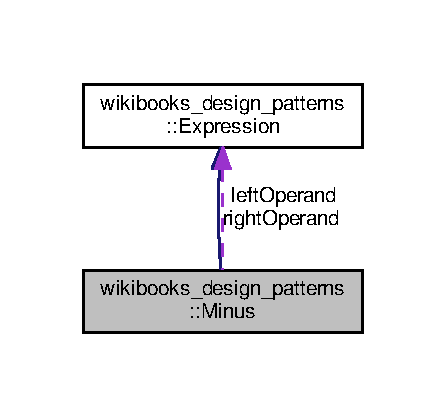
\includegraphics[width=214pt]{classwikibooks__design__patterns_1_1Minus__coll__graph}
\end{center}
\end{figure}
\subsection*{Public Member Functions}
\begin{DoxyCompactItemize}
\item 
\hyperlink{classwikibooks__design__patterns_1_1Minus_aded0c8005567ff815dc4ecf6053db1d7}{Minus} (\hyperlink{structwikibooks__design__patterns_1_1Expression}{Expression} $\ast$left, \hyperlink{structwikibooks__design__patterns_1_1Expression}{Expression} $\ast$right)
\item 
\hyperlink{classwikibooks__design__patterns_1_1Minus_adb1a9cef8d8bfa63f15a7c53c4da2787}{$\sim$\+Minus} ()
\item 
int \hyperlink{classwikibooks__design__patterns_1_1Minus_a6f2e1d5e4281ecee45dff5859af3978f}{interpret} (\hyperlink{namespacewikibooks__design__patterns_adf1889a865861dea765d8a115cc66ae9}{Map} variables)
\end{DoxyCompactItemize}
\subsection*{Private Attributes}
\begin{DoxyCompactItemize}
\item 
\hyperlink{structwikibooks__design__patterns_1_1Expression}{Expression} $\ast$ \hyperlink{classwikibooks__design__patterns_1_1Minus_af0a888e3e728165e0142bf230f0c2366}{left\+Operand}
\item 
\hyperlink{structwikibooks__design__patterns_1_1Expression}{Expression} $\ast$ \hyperlink{classwikibooks__design__patterns_1_1Minus_af555c67688bb374cb76ed7d99aa67220}{right\+Operand}
\end{DoxyCompactItemize}


\subsection{Constructor \& Destructor Documentation}
\index{wikibooks\+\_\+design\+\_\+patterns\+::\+Minus@{wikibooks\+\_\+design\+\_\+patterns\+::\+Minus}!Minus@{Minus}}
\index{Minus@{Minus}!wikibooks\+\_\+design\+\_\+patterns\+::\+Minus@{wikibooks\+\_\+design\+\_\+patterns\+::\+Minus}}
\subsubsection[{\texorpdfstring{Minus(\+Expression $\ast$left, Expression $\ast$right)}{Minus(Expression *left, Expression *right)}}]{\setlength{\rightskip}{0pt plus 5cm}wikibooks\+\_\+design\+\_\+patterns\+::\+Minus\+::\+Minus (
\begin{DoxyParamCaption}
\item[{{\bf Expression} $\ast$}]{left, }
\item[{{\bf Expression} $\ast$}]{right}
\end{DoxyParamCaption}
)\hspace{0.3cm}{\ttfamily [inline]}}\hypertarget{classwikibooks__design__patterns_1_1Minus_aded0c8005567ff815dc4ecf6053db1d7}{}\label{classwikibooks__design__patterns_1_1Minus_aded0c8005567ff815dc4ecf6053db1d7}

\begin{DoxyCode}
53                                                \{ 
54         \hyperlink{classwikibooks__design__patterns_1_1Minus_af0a888e3e728165e0142bf230f0c2366}{leftOperand} = left; 
55         \hyperlink{classwikibooks__design__patterns_1_1Minus_af555c67688bb374cb76ed7d99aa67220}{rightOperand} = right;
56     \}
\end{DoxyCode}
\index{wikibooks\+\_\+design\+\_\+patterns\+::\+Minus@{wikibooks\+\_\+design\+\_\+patterns\+::\+Minus}!````~Minus@{$\sim$\+Minus}}
\index{````~Minus@{$\sim$\+Minus}!wikibooks\+\_\+design\+\_\+patterns\+::\+Minus@{wikibooks\+\_\+design\+\_\+patterns\+::\+Minus}}
\subsubsection[{\texorpdfstring{$\sim$\+Minus()}{~Minus()}}]{\setlength{\rightskip}{0pt plus 5cm}wikibooks\+\_\+design\+\_\+patterns\+::\+Minus\+::$\sim$\+Minus (
\begin{DoxyParamCaption}
{}
\end{DoxyParamCaption}
)\hspace{0.3cm}{\ttfamily [inline]}}\hypertarget{classwikibooks__design__patterns_1_1Minus_adb1a9cef8d8bfa63f15a7c53c4da2787}{}\label{classwikibooks__design__patterns_1_1Minus_adb1a9cef8d8bfa63f15a7c53c4da2787}

\begin{DoxyCode}
57             \{ 
58     \textcolor{keyword}{delete} \hyperlink{classwikibooks__design__patterns_1_1Minus_af0a888e3e728165e0142bf230f0c2366}{leftOperand};
59     \textcolor{keyword}{delete} \hyperlink{classwikibooks__design__patterns_1_1Minus_af555c67688bb374cb76ed7d99aa67220}{rightOperand};
60     \}
\end{DoxyCode}


\subsection{Member Function Documentation}
\index{wikibooks\+\_\+design\+\_\+patterns\+::\+Minus@{wikibooks\+\_\+design\+\_\+patterns\+::\+Minus}!interpret@{interpret}}
\index{interpret@{interpret}!wikibooks\+\_\+design\+\_\+patterns\+::\+Minus@{wikibooks\+\_\+design\+\_\+patterns\+::\+Minus}}
\subsubsection[{\texorpdfstring{interpret(\+Map variables)}{interpret(Map variables)}}]{\setlength{\rightskip}{0pt plus 5cm}int wikibooks\+\_\+design\+\_\+patterns\+::\+Minus\+::interpret (
\begin{DoxyParamCaption}
\item[{{\bf Map}}]{variables}
\end{DoxyParamCaption}
)\hspace{0.3cm}{\ttfamily [inline]}, {\ttfamily [virtual]}}\hypertarget{classwikibooks__design__patterns_1_1Minus_a6f2e1d5e4281ecee45dff5859af3978f}{}\label{classwikibooks__design__patterns_1_1Minus_a6f2e1d5e4281ecee45dff5859af3978f}


Implements \hyperlink{structwikibooks__design__patterns_1_1Expression_a3723a35bb367b43edf806be72385c680}{wikibooks\+\_\+design\+\_\+patterns\+::\+Expression}.


\begin{DoxyCode}
62                                   \{ 
63         \textcolor{keywordflow}{return} \hyperlink{classwikibooks__design__patterns_1_1Minus_af0a888e3e728165e0142bf230f0c2366}{leftOperand}->\hyperlink{structwikibooks__design__patterns_1_1Expression_a3723a35bb367b43edf806be72385c680}{interpret}(variables) - 
      \hyperlink{classwikibooks__design__patterns_1_1Minus_af555c67688bb374cb76ed7d99aa67220}{rightOperand}->\hyperlink{structwikibooks__design__patterns_1_1Expression_a3723a35bb367b43edf806be72385c680}{interpret}(variables);
64     \}
\end{DoxyCode}


Here is the call graph for this function\+:
\nopagebreak
\begin{figure}[H]
\begin{center}
\leavevmode
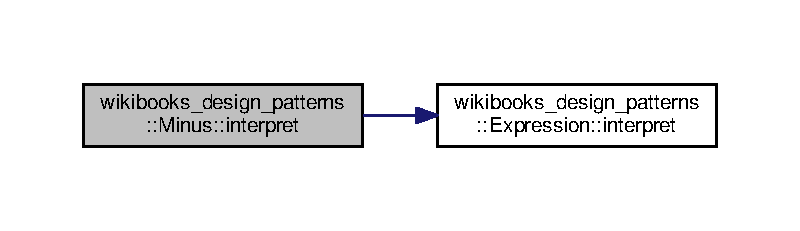
\includegraphics[width=350pt]{classwikibooks__design__patterns_1_1Minus_a6f2e1d5e4281ecee45dff5859af3978f_cgraph}
\end{center}
\end{figure}




\subsection{Member Data Documentation}
\index{wikibooks\+\_\+design\+\_\+patterns\+::\+Minus@{wikibooks\+\_\+design\+\_\+patterns\+::\+Minus}!left\+Operand@{left\+Operand}}
\index{left\+Operand@{left\+Operand}!wikibooks\+\_\+design\+\_\+patterns\+::\+Minus@{wikibooks\+\_\+design\+\_\+patterns\+::\+Minus}}
\subsubsection[{\texorpdfstring{left\+Operand}{leftOperand}}]{\setlength{\rightskip}{0pt plus 5cm}{\bf Expression}$\ast$ wikibooks\+\_\+design\+\_\+patterns\+::\+Minus\+::left\+Operand\hspace{0.3cm}{\ttfamily [private]}}\hypertarget{classwikibooks__design__patterns_1_1Minus_af0a888e3e728165e0142bf230f0c2366}{}\label{classwikibooks__design__patterns_1_1Minus_af0a888e3e728165e0142bf230f0c2366}
\index{wikibooks\+\_\+design\+\_\+patterns\+::\+Minus@{wikibooks\+\_\+design\+\_\+patterns\+::\+Minus}!right\+Operand@{right\+Operand}}
\index{right\+Operand@{right\+Operand}!wikibooks\+\_\+design\+\_\+patterns\+::\+Minus@{wikibooks\+\_\+design\+\_\+patterns\+::\+Minus}}
\subsubsection[{\texorpdfstring{right\+Operand}{rightOperand}}]{\setlength{\rightskip}{0pt plus 5cm}{\bf Expression}$\ast$ wikibooks\+\_\+design\+\_\+patterns\+::\+Minus\+::right\+Operand\hspace{0.3cm}{\ttfamily [private]}}\hypertarget{classwikibooks__design__patterns_1_1Minus_af555c67688bb374cb76ed7d99aa67220}{}\label{classwikibooks__design__patterns_1_1Minus_af555c67688bb374cb76ed7d99aa67220}


The documentation for this class was generated from the following file\+:\begin{DoxyCompactItemize}
\item 
\hyperlink{Interpreter_8cpp}{Interpreter.\+cpp}\end{DoxyCompactItemize}

\hypertarget{classwikibooks__design__patterns_1_1Number}{}\section{wikibooks\+\_\+design\+\_\+patterns\+:\+:Number Class Reference}
\label{classwikibooks__design__patterns_1_1Number}\index{wikibooks\+\_\+design\+\_\+patterns\+::\+Number@{wikibooks\+\_\+design\+\_\+patterns\+::\+Number}}


Inheritance diagram for wikibooks\+\_\+design\+\_\+patterns\+:\+:Number\+:
\nopagebreak
\begin{figure}[H]
\begin{center}
\leavevmode
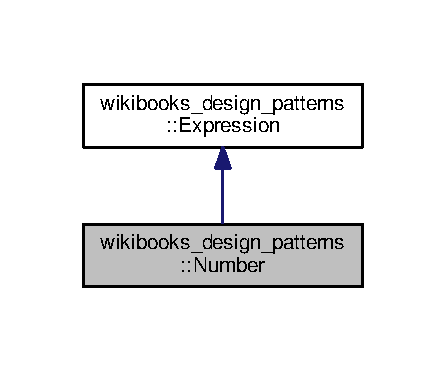
\includegraphics[width=214pt]{classwikibooks__design__patterns_1_1Number__inherit__graph}
\end{center}
\end{figure}


Collaboration diagram for wikibooks\+\_\+design\+\_\+patterns\+:\+:Number\+:
\nopagebreak
\begin{figure}[H]
\begin{center}
\leavevmode
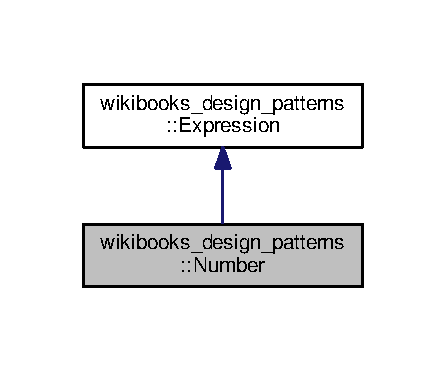
\includegraphics[width=214pt]{classwikibooks__design__patterns_1_1Number__coll__graph}
\end{center}
\end{figure}
\subsection*{Public Member Functions}
\begin{DoxyCompactItemize}
\item 
\hyperlink{classwikibooks__design__patterns_1_1Number_a3330cb7da5d43b43e02fc4ee1c39bf44}{Number} (int \hyperlink{classwikibooks__design__patterns_1_1Number_aef987597017592f4cdab36541b430778}{number})
\item 
int \hyperlink{classwikibooks__design__patterns_1_1Number_aed3e0a829546568864db2b8e5b667c72}{interpret} (\hyperlink{namespacewikibooks__design__patterns_adf1889a865861dea765d8a115cc66ae9}{Map} variables)
\item 
void \hyperlink{classwikibooks__design__patterns_1_1Number_ae829e1b9f618313c60c70e904a59ca53}{print\+Num} ()
\end{DoxyCompactItemize}
\subsection*{Private Attributes}
\begin{DoxyCompactItemize}
\item 
int \hyperlink{classwikibooks__design__patterns_1_1Number_aef987597017592f4cdab36541b430778}{number}
\end{DoxyCompactItemize}


\subsection{Constructor \& Destructor Documentation}
\index{wikibooks\+\_\+design\+\_\+patterns\+::\+Number@{wikibooks\+\_\+design\+\_\+patterns\+::\+Number}!Number@{Number}}
\index{Number@{Number}!wikibooks\+\_\+design\+\_\+patterns\+::\+Number@{wikibooks\+\_\+design\+\_\+patterns\+::\+Number}}
\subsubsection[{\texorpdfstring{Number(int number)}{Number(int number)}}]{\setlength{\rightskip}{0pt plus 5cm}wikibooks\+\_\+design\+\_\+patterns\+::\+Number\+::\+Number (
\begin{DoxyParamCaption}
\item[{int}]{number}
\end{DoxyParamCaption}
)\hspace{0.3cm}{\ttfamily [inline]}}\hypertarget{classwikibooks__design__patterns_1_1Number_a3330cb7da5d43b43e02fc4ee1c39bf44}{}\label{classwikibooks__design__patterns_1_1Number_a3330cb7da5d43b43e02fc4ee1c39bf44}

\begin{DoxyCode}
25 \{ this->\hyperlink{classwikibooks__design__patterns_1_1Number_aef987597017592f4cdab36541b430778}{number} = \hyperlink{classwikibooks__design__patterns_1_1Number_aef987597017592f4cdab36541b430778}{number}; \}
\end{DoxyCode}


\subsection{Member Function Documentation}
\index{wikibooks\+\_\+design\+\_\+patterns\+::\+Number@{wikibooks\+\_\+design\+\_\+patterns\+::\+Number}!interpret@{interpret}}
\index{interpret@{interpret}!wikibooks\+\_\+design\+\_\+patterns\+::\+Number@{wikibooks\+\_\+design\+\_\+patterns\+::\+Number}}
\subsubsection[{\texorpdfstring{interpret(\+Map variables)}{interpret(Map variables)}}]{\setlength{\rightskip}{0pt plus 5cm}int wikibooks\+\_\+design\+\_\+patterns\+::\+Number\+::interpret (
\begin{DoxyParamCaption}
\item[{{\bf Map}}]{variables}
\end{DoxyParamCaption}
)\hspace{0.3cm}{\ttfamily [inline]}, {\ttfamily [virtual]}}\hypertarget{classwikibooks__design__patterns_1_1Number_aed3e0a829546568864db2b8e5b667c72}{}\label{classwikibooks__design__patterns_1_1Number_aed3e0a829546568864db2b8e5b667c72}


Implements \hyperlink{structwikibooks__design__patterns_1_1Expression_a3723a35bb367b43edf806be72385c680}{wikibooks\+\_\+design\+\_\+patterns\+::\+Expression}.


\begin{DoxyCode}
26 \{ \textcolor{keywordflow}{return} \hyperlink{classwikibooks__design__patterns_1_1Number_aef987597017592f4cdab36541b430778}{number}; \}
\end{DoxyCode}
\index{wikibooks\+\_\+design\+\_\+patterns\+::\+Number@{wikibooks\+\_\+design\+\_\+patterns\+::\+Number}!print\+Num@{print\+Num}}
\index{print\+Num@{print\+Num}!wikibooks\+\_\+design\+\_\+patterns\+::\+Number@{wikibooks\+\_\+design\+\_\+patterns\+::\+Number}}
\subsubsection[{\texorpdfstring{print\+Num()}{printNum()}}]{\setlength{\rightskip}{0pt plus 5cm}void wikibooks\+\_\+design\+\_\+patterns\+::\+Number\+::print\+Num (
\begin{DoxyParamCaption}
{}
\end{DoxyParamCaption}
)\hspace{0.3cm}{\ttfamily [inline]}}\hypertarget{classwikibooks__design__patterns_1_1Number_ae829e1b9f618313c60c70e904a59ca53}{}\label{classwikibooks__design__patterns_1_1Number_ae829e1b9f618313c60c70e904a59ca53}

\begin{DoxyCode}
27 \{ cout << \hyperlink{classwikibooks__design__patterns_1_1Number_aef987597017592f4cdab36541b430778}{number}; \}
\end{DoxyCode}


\subsection{Member Data Documentation}
\index{wikibooks\+\_\+design\+\_\+patterns\+::\+Number@{wikibooks\+\_\+design\+\_\+patterns\+::\+Number}!number@{number}}
\index{number@{number}!wikibooks\+\_\+design\+\_\+patterns\+::\+Number@{wikibooks\+\_\+design\+\_\+patterns\+::\+Number}}
\subsubsection[{\texorpdfstring{number}{number}}]{\setlength{\rightskip}{0pt plus 5cm}int wikibooks\+\_\+design\+\_\+patterns\+::\+Number\+::number\hspace{0.3cm}{\ttfamily [private]}}\hypertarget{classwikibooks__design__patterns_1_1Number_aef987597017592f4cdab36541b430778}{}\label{classwikibooks__design__patterns_1_1Number_aef987597017592f4cdab36541b430778}


The documentation for this class was generated from the following file\+:\begin{DoxyCompactItemize}
\item 
\hyperlink{Interpreter_8cpp}{Interpreter.\+cpp}\end{DoxyCompactItemize}

\hypertarget{classwikibooks__design__patterns_1_1Plus}{}\section{wikibooks\+\_\+design\+\_\+patterns\+:\+:Plus Class Reference}
\label{classwikibooks__design__patterns_1_1Plus}\index{wikibooks\+\_\+design\+\_\+patterns\+::\+Plus@{wikibooks\+\_\+design\+\_\+patterns\+::\+Plus}}


Inheritance diagram for wikibooks\+\_\+design\+\_\+patterns\+:\+:Plus\+:
\nopagebreak
\begin{figure}[H]
\begin{center}
\leavevmode
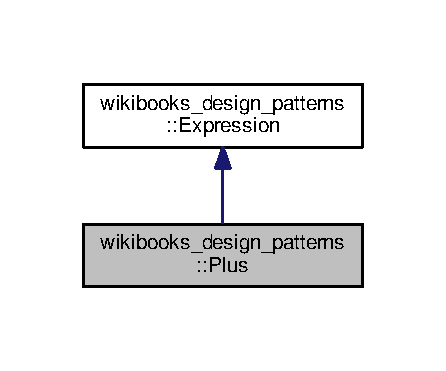
\includegraphics[width=214pt]{classwikibooks__design__patterns_1_1Plus__inherit__graph}
\end{center}
\end{figure}


Collaboration diagram for wikibooks\+\_\+design\+\_\+patterns\+:\+:Plus\+:
\nopagebreak
\begin{figure}[H]
\begin{center}
\leavevmode
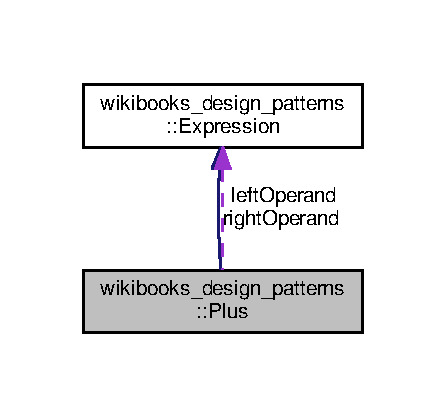
\includegraphics[width=214pt]{classwikibooks__design__patterns_1_1Plus__coll__graph}
\end{center}
\end{figure}
\subsection*{Public Member Functions}
\begin{DoxyCompactItemize}
\item 
\hyperlink{classwikibooks__design__patterns_1_1Plus_a97354a3768fce729287bbfa7a89d407c}{Plus} (\hyperlink{structwikibooks__design__patterns_1_1Expression}{Expression} $\ast$left, \hyperlink{structwikibooks__design__patterns_1_1Expression}{Expression} $\ast$right)
\item 
\hyperlink{classwikibooks__design__patterns_1_1Plus_ac6474c579f8814505b3b6882cb3116db}{$\sim$\+Plus} ()
\item 
int \hyperlink{classwikibooks__design__patterns_1_1Plus_a014d62447a10ada652b67da3fd2d6e4a}{interpret} (\hyperlink{namespacewikibooks__design__patterns_adf1889a865861dea765d8a115cc66ae9}{Map} variables)
\end{DoxyCompactItemize}
\subsection*{Private Attributes}
\begin{DoxyCompactItemize}
\item 
\hyperlink{structwikibooks__design__patterns_1_1Expression}{Expression} $\ast$ \hyperlink{classwikibooks__design__patterns_1_1Plus_a25d07e0b68a4c574974de8656f43230e}{left\+Operand}
\item 
\hyperlink{structwikibooks__design__patterns_1_1Expression}{Expression} $\ast$ \hyperlink{classwikibooks__design__patterns_1_1Plus_a8b54c7b23f28495c095b0d3e146094ea}{right\+Operand}
\end{DoxyCompactItemize}


\subsection{Constructor \& Destructor Documentation}
\index{wikibooks\+\_\+design\+\_\+patterns\+::\+Plus@{wikibooks\+\_\+design\+\_\+patterns\+::\+Plus}!Plus@{Plus}}
\index{Plus@{Plus}!wikibooks\+\_\+design\+\_\+patterns\+::\+Plus@{wikibooks\+\_\+design\+\_\+patterns\+::\+Plus}}
\subsubsection[{\texorpdfstring{Plus(\+Expression $\ast$left, Expression $\ast$right)}{Plus(Expression *left, Expression *right)}}]{\setlength{\rightskip}{0pt plus 5cm}wikibooks\+\_\+design\+\_\+patterns\+::\+Plus\+::\+Plus (
\begin{DoxyParamCaption}
\item[{{\bf Expression} $\ast$}]{left, }
\item[{{\bf Expression} $\ast$}]{right}
\end{DoxyParamCaption}
)\hspace{0.3cm}{\ttfamily [inline]}}\hypertarget{classwikibooks__design__patterns_1_1Plus_a97354a3768fce729287bbfa7a89d407c}{}\label{classwikibooks__design__patterns_1_1Plus_a97354a3768fce729287bbfa7a89d407c}

\begin{DoxyCode}
35                                               \{ 
36         \hyperlink{classwikibooks__design__patterns_1_1Plus_a25d07e0b68a4c574974de8656f43230e}{leftOperand} = left; 
37         \hyperlink{classwikibooks__design__patterns_1_1Plus_a8b54c7b23f28495c095b0d3e146094ea}{rightOperand} = right;
38     \}
\end{DoxyCode}
\index{wikibooks\+\_\+design\+\_\+patterns\+::\+Plus@{wikibooks\+\_\+design\+\_\+patterns\+::\+Plus}!````~Plus@{$\sim$\+Plus}}
\index{````~Plus@{$\sim$\+Plus}!wikibooks\+\_\+design\+\_\+patterns\+::\+Plus@{wikibooks\+\_\+design\+\_\+patterns\+::\+Plus}}
\subsubsection[{\texorpdfstring{$\sim$\+Plus()}{~Plus()}}]{\setlength{\rightskip}{0pt plus 5cm}wikibooks\+\_\+design\+\_\+patterns\+::\+Plus\+::$\sim$\+Plus (
\begin{DoxyParamCaption}
{}
\end{DoxyParamCaption}
)\hspace{0.3cm}{\ttfamily [inline]}}\hypertarget{classwikibooks__design__patterns_1_1Plus_ac6474c579f8814505b3b6882cb3116db}{}\label{classwikibooks__design__patterns_1_1Plus_ac6474c579f8814505b3b6882cb3116db}

\begin{DoxyCode}
39            \{ 
40     \textcolor{keyword}{delete} \hyperlink{classwikibooks__design__patterns_1_1Plus_a25d07e0b68a4c574974de8656f43230e}{leftOperand};
41     \textcolor{keyword}{delete} \hyperlink{classwikibooks__design__patterns_1_1Plus_a8b54c7b23f28495c095b0d3e146094ea}{rightOperand};
42     \}
\end{DoxyCode}


\subsection{Member Function Documentation}
\index{wikibooks\+\_\+design\+\_\+patterns\+::\+Plus@{wikibooks\+\_\+design\+\_\+patterns\+::\+Plus}!interpret@{interpret}}
\index{interpret@{interpret}!wikibooks\+\_\+design\+\_\+patterns\+::\+Plus@{wikibooks\+\_\+design\+\_\+patterns\+::\+Plus}}
\subsubsection[{\texorpdfstring{interpret(\+Map variables)}{interpret(Map variables)}}]{\setlength{\rightskip}{0pt plus 5cm}int wikibooks\+\_\+design\+\_\+patterns\+::\+Plus\+::interpret (
\begin{DoxyParamCaption}
\item[{{\bf Map}}]{variables}
\end{DoxyParamCaption}
)\hspace{0.3cm}{\ttfamily [inline]}, {\ttfamily [virtual]}}\hypertarget{classwikibooks__design__patterns_1_1Plus_a014d62447a10ada652b67da3fd2d6e4a}{}\label{classwikibooks__design__patterns_1_1Plus_a014d62447a10ada652b67da3fd2d6e4a}


Implements \hyperlink{structwikibooks__design__patterns_1_1Expression_a3723a35bb367b43edf806be72385c680}{wikibooks\+\_\+design\+\_\+patterns\+::\+Expression}.


\begin{DoxyCode}
44                                   \{ 
45         \textcolor{keywordflow}{return} \hyperlink{classwikibooks__design__patterns_1_1Plus_a25d07e0b68a4c574974de8656f43230e}{leftOperand}->\hyperlink{structwikibooks__design__patterns_1_1Expression_a3723a35bb367b43edf806be72385c680}{interpret}(variables) + 
      \hyperlink{classwikibooks__design__patterns_1_1Plus_a8b54c7b23f28495c095b0d3e146094ea}{rightOperand}->\hyperlink{structwikibooks__design__patterns_1_1Expression_a3723a35bb367b43edf806be72385c680}{interpret}(variables);
46     \}
\end{DoxyCode}


Here is the call graph for this function\+:
\nopagebreak
\begin{figure}[H]
\begin{center}
\leavevmode
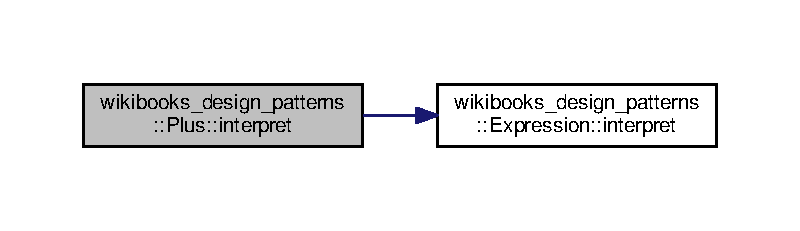
\includegraphics[width=350pt]{classwikibooks__design__patterns_1_1Plus_a014d62447a10ada652b67da3fd2d6e4a_cgraph}
\end{center}
\end{figure}




\subsection{Member Data Documentation}
\index{wikibooks\+\_\+design\+\_\+patterns\+::\+Plus@{wikibooks\+\_\+design\+\_\+patterns\+::\+Plus}!left\+Operand@{left\+Operand}}
\index{left\+Operand@{left\+Operand}!wikibooks\+\_\+design\+\_\+patterns\+::\+Plus@{wikibooks\+\_\+design\+\_\+patterns\+::\+Plus}}
\subsubsection[{\texorpdfstring{left\+Operand}{leftOperand}}]{\setlength{\rightskip}{0pt plus 5cm}{\bf Expression}$\ast$ wikibooks\+\_\+design\+\_\+patterns\+::\+Plus\+::left\+Operand\hspace{0.3cm}{\ttfamily [private]}}\hypertarget{classwikibooks__design__patterns_1_1Plus_a25d07e0b68a4c574974de8656f43230e}{}\label{classwikibooks__design__patterns_1_1Plus_a25d07e0b68a4c574974de8656f43230e}
\index{wikibooks\+\_\+design\+\_\+patterns\+::\+Plus@{wikibooks\+\_\+design\+\_\+patterns\+::\+Plus}!right\+Operand@{right\+Operand}}
\index{right\+Operand@{right\+Operand}!wikibooks\+\_\+design\+\_\+patterns\+::\+Plus@{wikibooks\+\_\+design\+\_\+patterns\+::\+Plus}}
\subsubsection[{\texorpdfstring{right\+Operand}{rightOperand}}]{\setlength{\rightskip}{0pt plus 5cm}{\bf Expression}$\ast$ wikibooks\+\_\+design\+\_\+patterns\+::\+Plus\+::right\+Operand\hspace{0.3cm}{\ttfamily [private]}}\hypertarget{classwikibooks__design__patterns_1_1Plus_a8b54c7b23f28495c095b0d3e146094ea}{}\label{classwikibooks__design__patterns_1_1Plus_a8b54c7b23f28495c095b0d3e146094ea}


The documentation for this class was generated from the following file\+:\begin{DoxyCompactItemize}
\item 
\hyperlink{Interpreter_8cpp}{Interpreter.\+cpp}\end{DoxyCompactItemize}

\hypertarget{classwikibooks__design__patterns_1_1Variable}{}\section{wikibooks\+\_\+design\+\_\+patterns\+:\+:Variable Class Reference}
\label{classwikibooks__design__patterns_1_1Variable}\index{wikibooks\+\_\+design\+\_\+patterns\+::\+Variable@{wikibooks\+\_\+design\+\_\+patterns\+::\+Variable}}


Inheritance diagram for wikibooks\+\_\+design\+\_\+patterns\+:\+:Variable\+:
\nopagebreak
\begin{figure}[H]
\begin{center}
\leavevmode
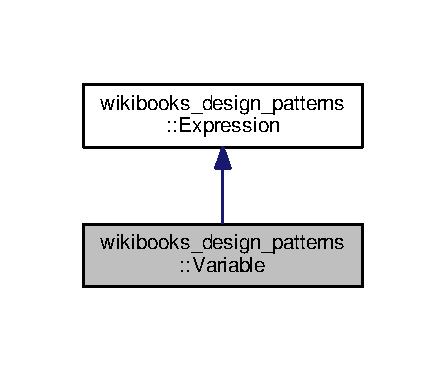
\includegraphics[width=214pt]{classwikibooks__design__patterns_1_1Variable__inherit__graph}
\end{center}
\end{figure}


Collaboration diagram for wikibooks\+\_\+design\+\_\+patterns\+:\+:Variable\+:
\nopagebreak
\begin{figure}[H]
\begin{center}
\leavevmode
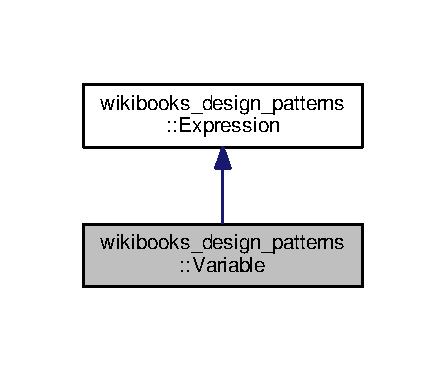
\includegraphics[width=214pt]{classwikibooks__design__patterns_1_1Variable__coll__graph}
\end{center}
\end{figure}
\subsection*{Public Member Functions}
\begin{DoxyCompactItemize}
\item 
\hyperlink{classwikibooks__design__patterns_1_1Variable_af253b16d4857b12246ef05128e21fa7f}{Variable} (\hyperlink{namespacewikibooks__design__patterns_a603d2591ea56686888d0e4389481a453}{String} \hyperlink{classwikibooks__design__patterns_1_1Variable_a68aaf6361a65a56622f5b91661921413}{name})
\item 
int \hyperlink{classwikibooks__design__patterns_1_1Variable_a4b0fe47e343d6991a62ee6b0d2179e2f}{interpret} (\hyperlink{namespacewikibooks__design__patterns_adf1889a865861dea765d8a115cc66ae9}{Map} variables)
\end{DoxyCompactItemize}
\subsection*{Private Attributes}
\begin{DoxyCompactItemize}
\item 
\hyperlink{namespacewikibooks__design__patterns_a603d2591ea56686888d0e4389481a453}{String} \hyperlink{classwikibooks__design__patterns_1_1Variable_a68aaf6361a65a56622f5b91661921413}{name}
\end{DoxyCompactItemize}


\subsection{Constructor \& Destructor Documentation}
\index{wikibooks\+\_\+design\+\_\+patterns\+::\+Variable@{wikibooks\+\_\+design\+\_\+patterns\+::\+Variable}!Variable@{Variable}}
\index{Variable@{Variable}!wikibooks\+\_\+design\+\_\+patterns\+::\+Variable@{wikibooks\+\_\+design\+\_\+patterns\+::\+Variable}}
\subsubsection[{\texorpdfstring{Variable(\+String name)}{Variable(String name)}}]{\setlength{\rightskip}{0pt plus 5cm}wikibooks\+\_\+design\+\_\+patterns\+::\+Variable\+::\+Variable (
\begin{DoxyParamCaption}
\item[{{\bf String}}]{name}
\end{DoxyParamCaption}
)\hspace{0.3cm}{\ttfamily [inline]}}\hypertarget{classwikibooks__design__patterns_1_1Variable_af253b16d4857b12246ef05128e21fa7f}{}\label{classwikibooks__design__patterns_1_1Variable_af253b16d4857b12246ef05128e21fa7f}

\begin{DoxyCode}
70 \{ this->\hyperlink{classwikibooks__design__patterns_1_1Variable_a68aaf6361a65a56622f5b91661921413}{name} = \hyperlink{classwikibooks__design__patterns_1_1Variable_a68aaf6361a65a56622f5b91661921413}{name}; \}
\end{DoxyCode}


\subsection{Member Function Documentation}
\index{wikibooks\+\_\+design\+\_\+patterns\+::\+Variable@{wikibooks\+\_\+design\+\_\+patterns\+::\+Variable}!interpret@{interpret}}
\index{interpret@{interpret}!wikibooks\+\_\+design\+\_\+patterns\+::\+Variable@{wikibooks\+\_\+design\+\_\+patterns\+::\+Variable}}
\subsubsection[{\texorpdfstring{interpret(\+Map variables)}{interpret(Map variables)}}]{\setlength{\rightskip}{0pt plus 5cm}int wikibooks\+\_\+design\+\_\+patterns\+::\+Variable\+::interpret (
\begin{DoxyParamCaption}
\item[{{\bf Map}}]{variables}
\end{DoxyParamCaption}
)\hspace{0.3cm}{\ttfamily [inline]}, {\ttfamily [virtual]}}\hypertarget{classwikibooks__design__patterns_1_1Variable_a4b0fe47e343d6991a62ee6b0d2179e2f}{}\label{classwikibooks__design__patterns_1_1Variable_a4b0fe47e343d6991a62ee6b0d2179e2f}


Implements \hyperlink{structwikibooks__design__patterns_1_1Expression_a3723a35bb367b43edf806be72385c680}{wikibooks\+\_\+design\+\_\+patterns\+::\+Expression}.


\begin{DoxyCode}
71                                   \{ 
72         \textcolor{keywordflow}{if}(variables.end() == variables.find(\hyperlink{classwikibooks__design__patterns_1_1Variable_a68aaf6361a65a56622f5b91661921413}{name})) \textcolor{keywordflow}{return} 0;
73         \textcolor{keywordflow}{return} variables[\hyperlink{classwikibooks__design__patterns_1_1Variable_a68aaf6361a65a56622f5b91661921413}{name}]->interpret(variables); 
74     \}
\end{DoxyCode}


\subsection{Member Data Documentation}
\index{wikibooks\+\_\+design\+\_\+patterns\+::\+Variable@{wikibooks\+\_\+design\+\_\+patterns\+::\+Variable}!name@{name}}
\index{name@{name}!wikibooks\+\_\+design\+\_\+patterns\+::\+Variable@{wikibooks\+\_\+design\+\_\+patterns\+::\+Variable}}
\subsubsection[{\texorpdfstring{name}{name}}]{\setlength{\rightskip}{0pt plus 5cm}{\bf String} wikibooks\+\_\+design\+\_\+patterns\+::\+Variable\+::name\hspace{0.3cm}{\ttfamily [private]}}\hypertarget{classwikibooks__design__patterns_1_1Variable_a68aaf6361a65a56622f5b91661921413}{}\label{classwikibooks__design__patterns_1_1Variable_a68aaf6361a65a56622f5b91661921413}


The documentation for this class was generated from the following file\+:\begin{DoxyCompactItemize}
\item 
\hyperlink{Interpreter_8cpp}{Interpreter.\+cpp}\end{DoxyCompactItemize}

\chapter{File Documentation}
\hypertarget{Interpreter_8cpp}{}\section{Interpreter.\+cpp File Reference}
\label{Interpreter_8cpp}\index{Interpreter.\+cpp@{Interpreter.\+cpp}}
{\ttfamily \#include $<$iostream$>$}\\*
{\ttfamily \#include $<$string$>$}\\*
{\ttfamily \#include $<$map$>$}\\*
{\ttfamily \#include $<$list$>$}\\*
Include dependency graph for Interpreter.\+cpp\+:
\nopagebreak
\begin{figure}[H]
\begin{center}
\leavevmode
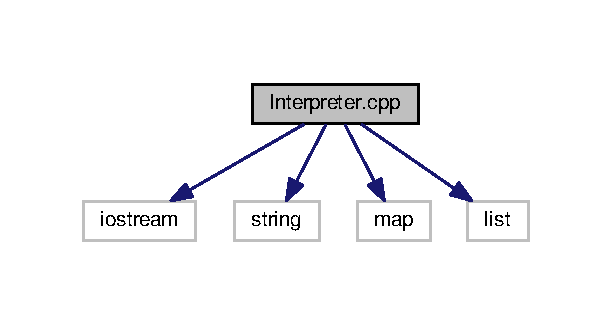
\includegraphics[width=294pt]{Interpreter_8cpp__incl}
\end{center}
\end{figure}
\subsection*{Classes}
\begin{DoxyCompactItemize}
\item 
struct \hyperlink{structwikibooks__design__patterns_1_1Expression}{wikibooks\+\_\+design\+\_\+patterns\+::\+Expression}
\item 
class \hyperlink{classwikibooks__design__patterns_1_1Number}{wikibooks\+\_\+design\+\_\+patterns\+::\+Number}
\item 
class \hyperlink{classwikibooks__design__patterns_1_1Plus}{wikibooks\+\_\+design\+\_\+patterns\+::\+Plus}
\item 
class \hyperlink{classwikibooks__design__patterns_1_1Minus}{wikibooks\+\_\+design\+\_\+patterns\+::\+Minus}
\item 
class \hyperlink{classwikibooks__design__patterns_1_1Variable}{wikibooks\+\_\+design\+\_\+patterns\+::\+Variable}
\item 
class \hyperlink{classwikibooks__design__patterns_1_1Evaluator}{wikibooks\+\_\+design\+\_\+patterns\+::\+Evaluator}
\end{DoxyCompactItemize}
\subsection*{Namespaces}
\begin{DoxyCompactItemize}
\item 
 \hyperlink{namespacewikibooks__design__patterns}{wikibooks\+\_\+design\+\_\+patterns}
\end{DoxyCompactItemize}
\subsection*{Typedefs}
\begin{DoxyCompactItemize}
\item 
typedef std\+::string \hyperlink{namespacewikibooks__design__patterns_a603d2591ea56686888d0e4389481a453}{wikibooks\+\_\+design\+\_\+patterns\+::\+String}
\item 
typedef std\+::map$<$ \hyperlink{namespacewikibooks__design__patterns_a603d2591ea56686888d0e4389481a453}{String}, \hyperlink{structwikibooks__design__patterns_1_1Expression}{Expression} $\ast$ $>$ \hyperlink{namespacewikibooks__design__patterns_adf1889a865861dea765d8a115cc66ae9}{wikibooks\+\_\+design\+\_\+patterns\+::\+Map}
\item 
typedef std\+::list$<$ \hyperlink{structwikibooks__design__patterns_1_1Expression}{Expression} $\ast$ $>$ \hyperlink{namespacewikibooks__design__patterns_a3247979de240b19de03793d4ec6ede0e}{wikibooks\+\_\+design\+\_\+patterns\+::\+Stack}
\end{DoxyCompactItemize}
\subsection*{Functions}
\begin{DoxyCompactItemize}
\item 
void \hyperlink{Interpreter_8cpp_acdef7a1fd863a6d3770c1268cb06add3}{main} ()
\end{DoxyCompactItemize}


\subsection{Function Documentation}
\index{Interpreter.\+cpp@{Interpreter.\+cpp}!main@{main}}
\index{main@{main}!Interpreter.\+cpp@{Interpreter.\+cpp}}
\subsubsection[{\texorpdfstring{main()}{main()}}]{\setlength{\rightskip}{0pt plus 5cm}void main (
\begin{DoxyParamCaption}
{}
\end{DoxyParamCaption}
)}\hypertarget{Interpreter_8cpp_acdef7a1fd863a6d3770c1268cb06add3}{}\label{Interpreter_8cpp_acdef7a1fd863a6d3770c1268cb06add3}

\begin{DoxyCode}
124 \{
125     \textcolor{keyword}{using namespace }\hyperlink{namespacewikibooks__design__patterns}{wikibooks\_design\_patterns};
126 
127     \hyperlink{classwikibooks__design__patterns_1_1Evaluator}{Evaluator} sentence(\textcolor{stringliteral}{"w x z - +"});
128 
129     \textcolor{keyword}{static}
130     \textcolor{keyword}{const} \textcolor{keywordtype}{int} sequences[][3] = \{
131         \{5, 10, 42\}, \{1, 3, 2\}, \{7, 9, -5\},
132     \};
133     \textcolor{keywordflow}{for} (\textcolor{keywordtype}{size\_t} i = 0; \textcolor{keyword}{sizeof}(sequences)/\textcolor{keyword}{sizeof}(sequences[0]) > i; ++i) \{
134         \hyperlink{namespacewikibooks__design__patterns_adf1889a865861dea765d8a115cc66ae9}{Map} variables;
135         variables[\textcolor{stringliteral}{"w"}] = \textcolor{keyword}{new} \hyperlink{classwikibooks__design__patterns_1_1Number}{Number}(sequences[i][0]);
136         variables[\textcolor{stringliteral}{"x"}] = \textcolor{keyword}{new} \hyperlink{classwikibooks__design__patterns_1_1Number}{Number}(sequences[i][1]);
137         variables[\textcolor{stringliteral}{"z"}] = \textcolor{keyword}{new} \hyperlink{classwikibooks__design__patterns_1_1Number}{Number}(sequences[i][2]);
138         \textcolor{keywordtype}{int} result = sentence.interpret(variables);
139         \textcolor{keywordflow}{for} (Map::iterator it = variables.begin(); variables.end() != it; ++it)
140         \{
141             \textcolor{keyword}{delete} it->second;
142         \}
143         std::cout<<\textcolor{stringliteral}{"Interpreter result: "}<<result<<std::endl;
144     \}
145 \}\end{DoxyCode}


Here is the call graph for this function\+:
\nopagebreak
\begin{figure}[H]
\begin{center}
\leavevmode
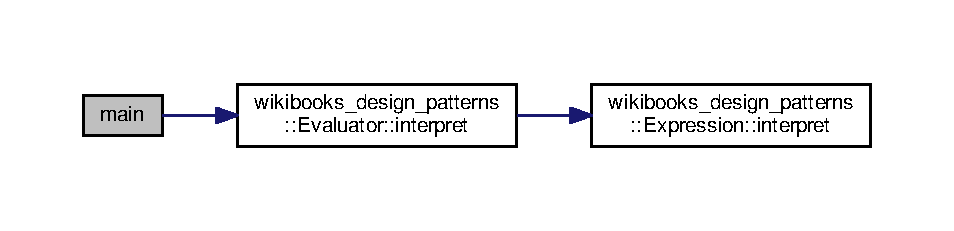
\includegraphics[width=350pt]{Interpreter_8cpp_acdef7a1fd863a6d3770c1268cb06add3_cgraph}
\end{center}
\end{figure}



%--- End generated contents ---

% Index
\backmatter
\newpage
\phantomsection
\clearemptydoublepage
\addcontentsline{toc}{chapter}{Index}
\printindex

\end{document}
